\documentclass[a4paper,12pt, german]{report}
\usepackage[german]{babel}
\usepackage[utf8]{inputenc}
\setcounter{tocdepth}{3}
\setcounter{secnumdepth}{3}

\usepackage{acro}

\DeclareAcronym{ki}{
  short = KI ,
  long  = künstliche Intelligenz
}



\usepackage{graphicx}
\usepackage{subcaption}
\usepackage{pdflscape}
\usepackage{array}
\usepackage{hhline,float}


\begin{document}
\title{Potentiale beim Einsatz künstlicher Intelligenz in der Produktion}
\author{Nathalie Becker}


\begin{titlepage}
\maketitle
\end{titlepage}


\begin{center}
\textbf{Abstract}
\end{center}
This is the Abstract


\tableofcontents
\printacronyms

\chapter{Einleitung}
%FAKT
In den letzten Jahren hat die Verwendung künstliche Intelligenz (KI) in der Wirtschaft und so auch in der Produktion stark zugenommen und trägt hier unter anderem zur Optimierung von Prozessen und zur Steigerung der Effizienz bei. Durch die Anwedung von Technologien, wie z.B. maschinellem Lernen oder Computer Vision bietet KI Möglichkeiten in der Produktion Probleme in Echtzeit zu erkennen und diese zu lösen, die Qualität von Produtken zu verbessern und auch die allgemeine Produktivitätzu erhöhen. Durch die zahlreichen Durchbrüche im Forschungsfeld der KI, ergeben sich laufend neue Potententiale für die Wirtschaft. 

Das Ziel dieser Arbeit ist es Potentiale von KI in der Produktion zu erarbeiten und zu bewerten. Hierfür wird zunächst ein Überblick sowohl über das Forschungsfeld und die Anwedungen der KI, als auch über den wirtschaftlichen Bereich der Produktion geschaffen. Nach der Beschreibung aktueller Beispiele von KI-Systemen in der Produktion, werden auf dieser Grundlage weitere mögliche Anwendungen aufgeführt und hinsichtlich der Wirtschaftlichkeit diskutiert.  

\chapter{Stand der Technik}

Das Forschungsgebiet der künstlichen Intelligenz ist breit gefächert und umfangreich. Der folgende Abschnitt gibt einen Einblick in diesen Bereich der Informatik. Auch das wirtschaftliche Feld der Prodktion wird in diesem Abschnitt beleuchtet.

\section{Künstliche Intelligenz}

Kaum eine Technologie bietet Grundlage für mehr Utopien und Dystropien als die künstliche Intelligenz. Filme in denen KI-Roboter die Welt übernehmen, eine Wirtschaft in der durch KI kaum mehr ein Mensch arbeiten muss oder der ..., sind Beispiele dafür. Was KI derzeit wirklich kann und in welchen Gebieten geforscht wird, wird in den kommenden Unterkapiteln aufgeführt.

\subsection{Grundlagen}

Künstliche Intelligenz (engl. Artificial Intelligence oder AI) ist ein Forschungzweig der Informatik und beschreibt eher einen Sammelbegriff als konkrete Disziplin oder Technologien. Grob geht es hier um technische Systeme, die selbstständig Lösungen für Probleme finden oder Entscheidungen treffen können. \cite{01} %\cite{10}

Die Definition der künstlichen Intelligenz ist in der Literatur uneindeutig. Schon für den Begriff der Intelligenz existiert keine allgemeingültige Definition und nur umstrittene Methoden zur Messung dieser. Über die letzten Jahrzehnte hat sich sowohl der Schwerpunkt des Forschungsgebietes, als auch dessen Zielsetzung immer wieder gewandelt. Ihren Ursprung fand die künstliche Intelligenz im Jahr 1955 mit der ersten Beschreibung durch John McCarthy:
\begin{quote}
  Ziel der KI ist es, Maschinen zu entwickeln, die sich verhalten, als verfügten sie über Intelligenz.
\end{quote}
 Mit der Schwierigkeit die Intelligenz an sich zu definieren, verliert diese Erklärung an Aussagenkraft. Elaine Rich bitet im Jahr 1983 eine weitere Möglichleit den Gegenstand der KI-Forschung zu benennen: 
 \begin{quote}
  Artificial Intelligence is the study of how to make computers do things at which, at the moment, humans are better.
 \end{quote} 
 Damit schafft Rich eine Beschreibung, die sowohl in der Vergangenheit, als auch in der Zukunft Anwendung findet. Beispielsweise sind Menschen bei Erkennen von Objekten, Menschen oder Sprachen den Maschinen noch weit überlegen. Bild- und Spracherkennung sind wichtige Forschungsbereiche der KI. Ein zentrales Gebiet der Forschung ist demnach auch das maschinelle Lernen, denn vorallem die Lernfähigkeit des Menschen durch Adaptivität stellt sich für Computer als Herausforderung dar.Dahingegen ist die Entwicklung von Schachcomputern nicht mehr relevant, denn diese sind bereits besser als der Mensch. Dennoch geht es bei KI nicht nur um praktische Implementierungen intelligenter Verfahren. Ein Teil des Forschungsgebietes befasst sich auch mit dem Verständnis des menschlichen Handelns und Schließens (Kognitionswissenschaft).
 %\cite{11}

Das KI-System ChatGPT des Unternehmens OpenAI beschreibt künstliche Intelligenz, also seinen eigenen Hintergrund so:
\begin{quote}
  Künstliche Intelligenz (KI) ist ein interdisziplinäres Gebiet, das sich mit der Entwicklung von Algorithmen und Systemen beschäftigt, die eine menschliche Intelligenz und kognititve Fähigkeiten imitieren. KI-Systeme können Aufgaben ausführen, die normalerweise nur von Menschen erledigt werden können, wie zum Beispiel das Verstehen von Sprache, das Erkennen von Gesichtern oder das Lösen komplexer Probleme.
\end{quote}

Chat GPT ist ein Chatbot, der Fragestellungen und Aufforderungen des Anwenders versteht und darauf antwortet bzw. die Aufgaben ausführt. Das Wissen ist allerdings nicht sein eigenes, denn er wurde mit großen Datenmengen trainiert, um diese Fähigkeit zu erlangen. Das beutet, dass dies nicht seine eigene Defintion ist, sondern vermutlich eine Kobination aus allen Erklärungen zum Thema KI mit dem das System trainiert wurde. Auf diesen Chatbot und der zugrundeliegenden Technologie wird in einem späteren Teil der Arbeit näher eingegangen.

Der Forschungsgegenstand und die Ziele der KI haben sich seit ihren Anfängen geändert. Während früher ausschließlich an Univerisäten mit Zielen wie der Entwicklung eines Schachcomputers, der dem Mensch überlegen ist, geforscht wurde, stehen heutzutage kommerzielle Anwendungen im Vordergrund. 
Gerade weil KI mittlerweile eine große Bedeutung in der Wirtschaft hat, wird mehr Geld in die Forschung investiert. So forschen nicht nur Universitäten, sondern auch andere Forschungsinstitute und Unternehmen in vielen Bereichen der KI. Auch die Verfügbarkeit von großen Datenmengen zu Trainingszwecken, die durch Verfahren der Daten-Analyse (Big-Data) für KI genutzt werden können, tragen einen großen Teil zu den zahlreichen Erfolgen der jüngeren Vergangenheit und Gegenwart bei. 

Zur näheren Begriffsklärung wird zwischen schwacher und starker KI unterschieden. Unter schwacher KI (auch "Narrow AI" oder "Special Purpose AI")  versteht man KI-Systeme, die für einen spezifischen Zweck, bzw. zur Lösung einer definierten Problematik entwicklet wurden. Sie können also Aufgaben ausführen, die sonst nur Menschen beweltigen können, meistens sogar schneller und effizierter. Allerdings sind sie nicht imstande kognititve Fähigkeiten eines Menschen zu imitieren. So sind Sprachassistenten wie Siri und Alexa in der Lage Sprachbefehle zu verstehen und auszuführen, sie besitzen aber keine emotionale Kompetenz oder die Fähigkeit komplexe Probleme zu lösen.
Im Gegensatz dazu wird bei starker KI eine komplette Nachbildung bzw. Imitation der menschlichen Intelligenz verstanden. Diese ist nicht nur auf ein Gebiet spezialisiert ist, sondern agiert gebietsübergreifend. Das bedeutet, diese verschieden Aufgaben ausführen könnte, für die bisher menschliche kognitive Föhrigkeiten nötig sind und dass Erkenntnisse aus einem Bereich auf andere Bereiche angewendet werden können. Damit könnten auch unbekannte Probleme durch die KI gelöst werden. Sie sind in der Lage ihre Umwelt zu verstehen und eigenständig zu lernen. In der aktuellen Forschung ist die Entwicklung ein starken KI jedoch nicht nicht absehbar und wird von manchen Experten soagr als unmöglich eingestuft. Bei der Entwicklung sollten außerdem mögliche Gefahren und ethische Aspekte berücksichtigt werden. 
Im Kotext dieser Arbeit und auch in weiten Teilen der Forschung und Anwendung wird von schwacher KI gesprochen.
% Abbildung schwache vs. starke KI

\subsection{Verfahren und Ansätze}

Nicht nur die Definition auch eine Segmentierung, Kategorisierung oder Einteilung der Technologien und Ansätze des umfangreichen und höchstdynamischen Forschungsgebietes der künstlichen Intelligenz ist nicht einfach und wird in der Literatur unterschiedlich vorgenommen. Diese Arbeit orientiert sich grob an der Kategorisierung des Trendsonar des ÖFIT aus dem Jahr 2018. Dieses unterteilt KI in die folgenden drei Bereiche: Lernmethoden, Technologien und Algorithmen, sowie Systeme und Architekturen. %\cite{öfit}
Diese Bereiche sind nicht vollständig voneinander zu trennen.  

\subsubsection{Lernmethoden}
Ein künstliche Intelligenz ist nicht von Beginn an intelligent. Sie muss lernen. Maschinelles Lernen (Machine Learning) ist eines der größten KI-Forschungsfelder. Anhand verschiedener Lernmethoden wird das technische System mit Daten trainiert wodurch erst die Fähigkeiten der KI entstehen. Die jeweilgen Ansätze sind für unterschiedliche Anwendungen geeignet. Dennoch bringen auch unkoventionelle Ansätze Durchbrüche in der Forschung. Folgend werden die relevantesten Methoden genannt und kurz beschrieben.


\paragraph{Supervised Learning (Überwachtes Lernen )} $ $ \\ Supervised Learning ist derzeit der am weitesten verbreitete Ansatz des Machine Learnings. Dabei werden bekannte Daten, sogenannte Trainigsdaten genutzt. Diese enthalten bereits Ergebnisse zu den jeweiligen Eingaben. Der Algorithmus erhält zunächst nur die Eingaben und triftt eine Entscheidung über die Ausgabe. Anschließend vergleicht er seine Aussagen mit dem vorgegebenen Ergebnis und passt seine nächste Beurteilung entsprechend an. Der Algortihmus wird so lange trainiert, bis nahezu immer die korrekte Entscheidung getroffen wurde. Dadurch soll der Algorithmus anschließend in der Lage sein Aussagen zu neuen, unbekannten Eingaben treffen zu können.

Beispielsweise werden dem Algortihmus unsortiert Bilder von Katzen und Hunden gezeigt. Er sieht während seiner Entscheidung aber nicht das jweilige Label "Katze" oder "Hund". Er entscheidet anhand des Bildes um welches der beiden Tiere es sich handelt und überprüft anschließend, ob seine Aussage korrekt war. So lernt der Algorithmus wie er Hund und Katzen untscheiden kann. Solche Algorthmien werden beispielsweise für Bilderkennungs-Systeme verwendet. 
%Abbildung

Diese Lernmethode wird gerne genutzt, da der Entwickler hier die Kontrolle über die Trainingsdaten, also den Input hat. Es ist von Anfang an klar, welches Ergbnis am Ende stehen soll. Allerdings nimmt diese Methode viel Zeit in Anspruch, da die Daten vor der Verwendung gelabelt werden müssen. Ein Problem dieser Methodik ist auch, dass der Algorithmus nur das lernt, was er mit den Inputdaten beigebracht bekommt. Wird ein Algortihmus beispielsweise nur mit Bildern von schwarzen Katzen trainiert, lernt er, dass eine Katze schwarzes Fell besitzt und wird eine weiße Katze nicht erkennen.

\paragraph{Unsupervised Learning (Unüberwachtes Lernen)} $  $ \\ Beim Unsupervised Learning versucht ein künstliches neuronales Netz (siehe unten) Zusammenhänge, Ähnlichkeiten, Strukturen und Muster innerhalb einer großen Menge an Eingabedaten zu erkennen. Der Algorithmus kann so beispielsweise zur Gruppierung (Clustering) von Daten oder zur Findung von Beziehungen (Association) genutzt werden.

Ein Beispiel für Clustering (K-Clustering) ist, wenn dem Algorithmus Bilder gegeben werde mit der Vorgabe, dass es sich hier um zwei (K=2) Arten von Tieren handelt: Hunde und Katzen. Der Algortihmus verucht also die Bilder über mehrere Itterationen nach Hunden und Katzen zu kategorisieren. So können in der Wirtschaft Daten genutzt werden, um z.B. Personengruppen zusammenzustellen, die für eine Marketingstrategie genutzt werden können.
% Abbildung

Associations werden genutzt, um Zusammenhänge zwischen den Daten zu finden. Ein Anwendung hierfür ist beispielsweise Amazon mit "Kunden, die diesen Artikel gekauft haben, kauften auch diesen Artikel".

Auch Sprachassistenten und Chatbots funktionieren mit Unsupervised Learning. Sie lernen durch die Interaktion mit Nutzern, wodurch Alexa oder Siri immer besser die Spracheingaben des Besitzers verstehen und Chatbots immer besser kommunizieren können. Mit welchen Daten der Algorithmus gefüttert wird, beeinflusst also die Ausgaben der KI. Ein Beispiel für ein Problematik, die sich aus dieser Methode ergibt, war 2016 der KI-Chatbot "Tay" von Microsoft. Dieser hatte Zugang zu Twitter. Innhalb von 24 Stunden entwickelten sich die zunächst einfältigen Aussagen der KI hin zu, Hetze gegen Ausländer und Feministen und der Verarbeitung von Verschwörungstheorien. Es ist allerdings nicht bekannt, ob Tay absichtlich von Nutzern mit diesen Daten gefüttert wurde. 




\paragraph{Reinforcement Learning (Bestärkendes Lernen)} $ $ \\ Das Reinforcement Learning ist die dritte Variante Algorithmen so zu trainieren, dass sie selbstständig Entscheidungen treffen können. Für diese Methoden werden allerdings keine Daten zum Lernen benötigt. Die Daten werden während des Trainigs selbst generiert und gelabelt. Der Algorithmus durchläuft dabei zahlreiche Itterationen um auf ein exaktes Ergebnis zu kommen. Es werden nur Impulse zur Unterstützung gesetzt. Ziel dieser Methode ist es, dass die KI in der Lage ist Probeleme zu lösen ohne dafür menschliches Vorwissen zu nutzen.
....%TPD




\paragraph{Deep Learning} %TBD
\paragraph{Meta-Lernen} %TBD

\subsubsection{Technologien und Algorithmen}
KI-Systeme werden aus Bausteinen, wie Technologien und Algorithmen zusammengesetzt. Es werden beispielsweise mathematische Methoden genutzt, um Daten zu klassifizieren und zu verarbeiten oder um Lösungen für Probleme zu finden und zu optimieren. Ein KI-System ensteht also durch die Kombination verschiedener Technologien und Optimierungsmethoden, wodurch spezielle, definierte Aufgaben gelöst werden können. Dies ermöglicht außerdem innovative Funktionalitäten. Einige dieser Bausteine sind hier aufgelistet.
%TBD

\subsubsection{Systeme und Architekturen}
Wie im oben beschrieben, entstehen KI-Systeme aus der Kombination von KI-Technologien, wodurch eine übergeordnete Funktion realisiert werden kann. Oft werden auch einzelne Komponenten der Systeme und Architekturen ausgetauscht und diese auf dem aktuellen Stand der Technik zu halten, oder um weitere Funktionalitäten zu ermöglichen. KI-Systeme können weiter in drei Kategorien unterteilt werden, wobei auch hier andere Einordnungen möglich sind:
%TBD


%Drei Kategrien: maschinelles Lernen, Regelbasierte KI, Künstliche neuronale Netze

\subsection{Anwendungen}
???


\section{Produktion}

Die Produktion ist eine der Grundfunktionen eines Unternehmens und ist verantwortlich für die Leistungserstellung. Sie hat einen großen Einfluss auf die Wirtschaftlichkeit. In diesem Abschnitt der Arbeit wird der Unternehmensbereich der Produktion näher beleuchtet.

\subsection{Grundlagen und Ziele der Produktion}

In der Produktion werden durch den gelenkten Einsatz von Produktionsfaktoren Güter oder Dienstleistungen hergestellt. %\cite{12}

\begin{figure}[H]
  \center
 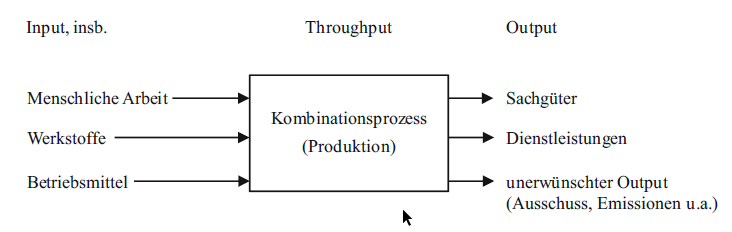
\includegraphics[width=9cm]{images/Kombinationsprozess.png}
  \caption[Kombinationsprozess der Produktion]{Kombinationsprozess der Produktion (leicht abgewandelt übernommen von) \cite{13}}
\end{figure}

Der Begriff der Produktionsfaktoren umfasst dabei alles was zur Leistungserstellung und zur Aufrechterhaltung und Ausbau der Leistungsbereitschaft dient. In der Volwirtschaftlehre bestehen dieser Faktoren aus Arbeit, Boden und Kapital. Dahingegen spricht die Betriebswirtschaftlehre von menschlicher Arbeit, Betriebsmittel und Werkstoffen (Produktionsfaktorsystem nach Gutenberg)

In der Wirtschaft lassen sich Ziele beispielsweise in monetäre und nicht monetäre Ziele unterteilen. Wobei sich monetäre Ziele unter anderem mit Kennzahlen wie Gewinn, Umsatz und Kostenminimierung beschreiben lassen und nicht-monetäre Ziele mit Produktivität, Qualität der Produkte und Kundenzufriedenheit. Auf all diese Ziele hat die Produktion einen großen Einfluss oder sind maßgeblich an der Erreichung beteiligt.

Übergeordnet werden in dieser Arbeit die Zielgrößen der Wirtschaftlichkeit und der Produktivität betrachtet. Die Wirtschaftlichkeit misst das Verhältnis zwischen Aufwand und Ertrag.
\begin{equation}
  Wirtschaftlichkeit =(Ertrag\frac{Aufwand})
\end{equation}


Sie umfasst die Planung, Steuerung, Organisation und Überwachung von Aktivitäten, die zur Leistungserstellung erforderlich sind. Diese werden im Folgenden anhand des Produtkionsprozessen dargestellt.


%-----------

Wirtschaftlichkeit ist eine wichtige ökonomische Zielgröße: Verhältnis Output zu Input
Produktivität Verhältnis Ausbringungsmeneg nud Faktoreinsatz (nur eine Produk- und Faktorart) (tech.Ziel)

"Zusammenfassend können als typische Ziele der Produktionswirtschaft geringe Kosten,
ein hoher Output, eine hohe Produktqualität, eine hohe Termineinhaltung und Auslastung
der Fertigungsbereiche (oder einzelner Maschinen) sowie geringe Durchlaufzeiten
genannt werden." Die Ziele fallen in unterschiedliche Planungsbereiche



\subsection{Produktionsprozess}

\subsubsection{Produktionsplanung}
- Prozess, Strategie

- Materialbedarf, Kapazitätsplanung, Zeitplanung
Produktionsprogramm: bestimmt in welcher Menge und art Produktionsfaktoren eingesetzt/beschafft werden müssen.

\subsubsection{Durchführung der Produktion}
Produktionsmethode: Fertigung, Montage
Steuerung: just in time, lean,...

\subsubsection{Kontrolle und Überwachung der Produktion}
Qualität, Lestungsmessung, Fehleranalyse, Zeit
\subsection{Herausforderungen und Schwierigekeiten}

- Engpässe
- Lieferschwierigkeiten
- Qualitätsprobleme
- Kostenprobleme


\chapter{Künstlicher Intelligenz in der Produktion}

Nachdem im vorangehenden Kapitel die Grundlagen der künstlichen Intelligenz, wie auch der Produktion geklärt wurden, werden diese beiden Themenfelder in den kommenden zwei Abschnitten zusammengeführt. In diesem Kapitel werden aktuelle Anwedungen der künstlichen Intelligenz in der Produktion beschrieben und bewertet. Die Bewertung findet in drei/vier Kategorien statt: Wirtschaftlichkeit, Risiken und Potentiale.

\section{Potentiale?? von KI in der Produktion}

- Erhöhung der Effizienz: Prozesse automatisieren, Produktionsleistungen überwachen und optimieren, Fehlerrate reduzieren, Effizienz und Produtivität in Produtkion erhöhen
- Steigerung der Qualität: Qualität überwachen und verbessern, indem Fehler und defekte automatisch erkannt und korrigiert werden, Erhöhung Kundenzufriedenheit
- Reduzierung von Kosten: Erhöhung der Effizienz/Produktivität steigern, Fehlerrate reduzieren, Verfügbarkeit der Anlage erhöhen
- Flexibilität und Anpassungfähigkeit: Prozesse schneller und flexibler an veränderte Bedingungen anpassen, zb Änderungen der Produktionsanforderungen, dadurch eff/Prod
- Predictive Maintantance: Zustand der Produktionsanlagenvorhersagen um Wartungsarbeiten gezielt durchzuführen, erhöht Verfügbarkeitder Anlagen und verringert Kosten für Reperaturen und Wartungsarbeiten

\section{Herausforderungen?}

\section{Anwedungsbeispiele}

\section{Potententiale}

\chapter{Fazit und Ausblick}

\listoffigures

\clearpage




\clearpage
\addcontentsline{toc}{chapter}{Literaturverzeichnis}

% Nochmal recherchieren wie man IEEE Standard im Literaturverzeichnis umsetzt


\begin{thebibliography}{99}

\bibitem{01}
	P. Buxmann, H. Schmidt,
	Künstliche Intelligenz: Mit Algorithmen zum wirtschaftlichen Erfolg,
	Springer Gabler,
	2.Auflage,
	2021.
	
\bibitem{02}
	A. Mockenhaupt,
	Digitalisierung und Künstliche Intelligenz in der Produktion: Grundlagen und Anwendung,
	Springer Vieweg,
	2021.

\bibitem{03}
	T. Kaufmann, H. Servatius,
	Das Internet der Dinge und Künstliche Intelligenz als Game Changer: Wege zu einem Management 4.0 und einer digitalen Architektur,
	Springer Vieweg,
	2020.

\bibitem{04} 	
	ChatGPT,
	OpenAI,
	Aufgerufen am 14.01.2023.

\bibitem{05}
	C. Appugliese, P. Nathan, W. S. Roberts
	Agil AI
	O´Reilly Media, Inc.,
	2020.

\bibitem{06}
	GI. Spindler,
	Produktion in Basiswissen Allgemeine Betriebswirtschaftslehre,
	p. 27-46,
	Springer Gabler,
	2022.

\bibitem{07}
	J. Bloech, R. Bogaschewsky, U. Buscher, A. Daub, U. Götze, F. Roland,
	Einführung in die Produktion,
	Springer Gabler, 
	2014.
	
\bibitem{08}
	I. Knappertsbusch, K. Gondlach,
	Arbeitswelt und KI 2030: Herausforderungen und Strategien für die Arbeit von morgen,
	Springer Gabler,
	2022.

\bibitem{09}
	R. Buchkremer, T. Heupel, O. Koch,
	Künstliche Intelligenz in Wirtschaft \& Gesellschaft: Auswirkungen, Herausforderungen \& Handlungsempfehlungen
	Springer Gabler,
	2020.

\bibitem{10}
	C. Welzel, D. Grosch,
	Das ÖFIT-Trendsonar Künstliche Intelligenz,
	Kompetenzzentrum Öffentliche Informationstechnologie,
	2018.

\bibitem{11}
	W. Ertel,
	Grundkurs Künstliche Intelligenz: Eine praxisorientierte Einführung,
	5. Auflage,
	Springer Vieweg,
	2021.

\bibitem{12}
	H. J. Wildermann, K. J. Schmidt,
	Produktion, 
	in: W. Lück, Lexikon der Betriebswirtschaft,
	Verlag moderne Industrie,
	1990.


\bibitem{15}
	T. Zwingmann,
	AI-Powered Business Intelligence,
	O'Reilly Media, Inc.,
	2022.

\bibitem{16}
	U.Walter,
	Künstliche Intelligenz für Dummies (Vortrag),
	Deutsches Museum München,
	https://www.youtube.com/watch?v=B7vCtHvYMyE
	2020.

\bibitem{17}
	D. Sonnet,
	Neuronale Netze kompakt: Vom Perceptron zum Deep Learning,
	Springer Vieweg,
	2022.

\bibitem{18}
	C. Steger, M. Ulrich, C. Wiedemann,
	Machine Vision Algorithms and Applications,
	Wiley-VCH,
	2018.

\bibitem{19}
	A. Jorzig, F. Sarangi,
	Künstliche Intelligenz und Robotik, 
	in: Digitalisierung im Gesundheitswesen,
	Springer,
	2020.

\bibitem{20}
	E. Gutenberg,
	Grundlagen der Betriebswirtschaftslehre, Band 1: Produktion,
	Springer,
	1951.




\end{thebibliography}

\appendix


\end{document}